\documentclass[10pt,a4paper]{article}
\usepackage[utf8]{inputenc}
\usepackage[margin=2cm]{geometry}
\usepackage{amsmath,amssymb}
\usepackage{graphicx}
\usepackage{booktabs,longtable,tabularx,makecell,multirow,array}
\usepackage{caption}
\usepackage{xcolor,colortbl}
\usepackage{tikz}
\usetikzlibrary{positioning,arrows.meta,calc}
\usepackage{fancyhdr}
\usepackage{xr}
\externaldocument{main}
\usepackage[hidelinks]{hyperref}
\newcommand{\seerLeakAUC}{0.735}
\newcommand{\seerLeakSD}{0.031}
\newcommand{\seerLeakCI}{0.701--0.768}
\newcommand{\seerLeakBE}{0.131 / 0.149}
\newcommand{\seerLeakECE}{0.149}
\newcommand{\seerPCAAUC}{0.735}
\newcommand{\seerPCASD}{0.031}
\newcommand{\seerPCACI}{0.701--0.768}
\newcommand{\seerPCABE}{0.131 / 0.149}
\newcommand{\seerPCAECE}{0.149}
\newcommand{\seerRFAUC}{0.741}
\newcommand{\seerRFSD}{0.027}
\newcommand{\seerRFCI}{0.713--0.770}
\newcommand{\seerRFBE}{0.130 / 0.146}
\newcommand{\seerRFECE}{0.146}
\newcommand{\seerUniAUC}{0.739}
\newcommand{\seerUniSD}{0.028}
\newcommand{\seerUniCI}{95\% CI 0.709--0.769}
\newcommand{\seerUniBE}{0.130 / 0.146}
\newcommand{\seerUniECE}{0.146}
\newcommand{\seerUniCIs}{0.709--0.769}
\newcommand{\seerUniP}{0.5607}
\newcommand{\seerUniTOST}{0.2251}
\newcommand{\seerCITL}{$-$1.00}
\newcommand{\seerSlope}{1.17}
\newcommand{\seerMeanPred}{28.6}
\newcommand{\seerDiffUL}{+0.0043}
\newcommand{\seerDiffULci}{$-$0.0082 to +0.0169}
\newcommand{\seerDiffPL}{+0.0000}
\newcommand{\seerDiffPLci}{$-$0.0014 to +0.0014}
\newcommand{\seerConfCov}{95.26}
\newcommand{\seerConfSingle}{61.92}
\newcommand{\seerConfAmb}{38.08}
\newcommand{\seerNcal}{556}
\newcommand{\seerNcalEv}{78}
\newcommand{\seerLbAcc}{83.50}
\newcommand{\seerLbAccCI}{79.96--86.52}
\newcommand{\seerLbBal}{63.73}
\newcommand{\seerLbSens}{36.23\% (25/69)}
\newcommand{\seerLbSpec}{91.23\% (385/422)}
\newcommand{\seerLbAUC}{0.722}
\newcommand{\seerLbAUCCI}{0.646--0.790}
\newcommand{\seerLbBrier}{0.132}
\newcommand{\seerLbBrierCI}{0.121--0.144}
\newcommand{\seerLbSlope}{1.03}
\newcommand{\seerLbSlopeCI}{0.69 to 1.41}
\newcommand{\seerLbInt}{$-$1.00}
\newcommand{\seerLbIntCI}{$-$1.22 to $-$0.78}
\newcommand{\seerLbCITL}{$-$1.02}
\newcommand{\seerLbCITLCI}{$-$1.10 to $-$0.94}
\newcommand{\seerLbCov}{95.32}
\newcommand{\seerLbCovCI}{93.07--96.86}
\newcommand{\wbcdLbBrier}{0.010}
\newcommand{\wbcdLbBrierCI}{0.004--0.017}
\newcommand{\seerRFfolds}{31}
\newcommand{\seerRFpct}{89}
\newcommand{\seerShapTop}{progesterone receptor status, N stage, number of positive regional nodes, age and histological grade}
\newcommand{\seerDCAlo}{0.09}
\newcommand{\seerDCAhi}{0.16}
\newcommand{\seerCovRange}{94.0\% to 96.5\%}
\newcommand{\seerMaxSMD}{$\le$0.08}
\newcommand{\seerNcompRange}{maximal fluctuation 0.0527 AUROC}
\newcommand{\seerFairText}{Discrimination was similar across racial groups (AUROC 0.738 White, 0.729 Black, 0.765 Other; overlapping CIs) but declined with age (0.774 for $<$50 years vs 0.699 for 60--69 years). Calibration differed markedly: the model overpredicted risk in all groups, but least for Black patients (CITL $-$0.40, 95\% CI $-$0.51 to $-$0.28; observed risk 24.4\% vs predicted 31.4\%) and most for Other-race patients (CITL $-$1.44; observed 8.6\% vs predicted 26.3\%). Because predicted risks varied much less between groups than observed risks, the model compressed the higher mortality of Black patients relative to other groups, so a single recalibration would not correct all groups equally. Sensitivity at the 0.5 threshold was lowest for Other-race (22.2\%) and Black (25.5\%) patients, and conformal coverage ranged from 94.0\% to 96.5\%. Subgroup sizes, particularly the 51 events among Black and 18 among Other-race patients, make these estimates imprecise.}

\newcommand{\seerMaxDeathMonth}{102}
\newcommand{\seerReproText}{reproduced all 35 outer-fold AUROC and accuracy values of the four pipelines reported in \texttt{results/SEER/SEER\_raw\_cv\_scores.csv} (maximum absolute difference 0 at the stored precision), and the Unified pipeline selected RF in 35/35 folds as in v1.0.}
\makeatletter\newcommand{\inputrows}[1]{\@@input #1 }\makeatother
\captionsetup{font=small,labelfont=bf}
\renewcommand{\thetable}{S\arabic{table}}
\renewcommand{\thefigure}{S\arabic{figure}}
\renewcommand{\labelitemi}{$\bullet$}
\pagestyle{fancy}\fancyhf{}
\lhead{\small\itshape TRUST-BC: Supplementary Material}\rhead{\small S\thepage}
\newcommand{\loc}[1]{Sec.~\ref{#1}, p.~\pageref{#1}}
\newcommand{\R}{\cellcolor{green!12}Reported}
\newcommand{\NA}{\cellcolor{gray!12}N/A}
\newcommand{\NR}{\cellcolor{orange!15}Not in abstract}
\newcommand{\PR}{\cellcolor{yellow!20}Partial}
\setlength{\parskip}{3pt}\setlength{\parindent}{0pt}

\renewcommand{\cellalign}{lc}
\newcolumntype{P}[1]{>{\raggedright\arraybackslash}p{#1}}
\newcolumntype{Y}{>{\raggedright\arraybackslash}X}
\begin{document}
\begin{center}
{\Large\bfseries Supplementary Material}\\[4pt]
{\large TRUST-BC: A Multicohort Benchmark for Leakage-Free, Calibrated, and Uncertainty-Aware Breast Cancer Prediction Models}\\[6pt]
Shayegan, Abolghasemi, Salehi, Kiarsi
\end{center}

\noindent Page numbers in the checklists refer to the PDF version of the revised main manuscript (section numbers are identical in the Word version). All tables in this document are also provided as CSV files in the repository folder \texttt{supplementary/tables/}, and every number can be regenerated with the scripts in \texttt{scripts/}.

\tableofcontents
\bigskip

\section*{S0. Contents of this supplement}
\addcontentsline{toc}{section}{S0. Contents of this supplement}
\begin{itemize}
\item Table S1: completed TRIPOD+AI checklist; Table S1b: TRIPOD+AI for Abstracts checklist.
\item Table S2: author self-assessment against PROBAST+AI (development and evaluation parts).
\item Figure S1: participant flow diagram.
\item Tables S3 and S3b: participant characteristics by partition and by race (SEER).
\item Table S4: number of participants and events in each analysis.
\item Table S5: Nadeau--Bengio corrected confidence intervals for all pipelines.
\item Table S6: conformal coverage by outcome class and subgroup (SEER).
\item Table S7: leakage and selector contrasts, all cohorts and label versions.
\item Section S8: SEER label audit, v1.0 results, reproduction check.
\item Table S9: minimum sample size (Riley criteria).
\end{itemize}

\newpage
\section*{Table S1. TRIPOD+AI checklist}
\addcontentsline{toc}{section}{Table S1. TRIPOD+AI checklist}
Item descriptions are abbreviated from the TRIPOD+AI statement (Collins et al., BMJ 2024;385:e078378). D = development, E = evaluation; this study reports both.

{\small
\begin{longtable}{@{}P{0.9cm}P{5.2cm}P{2.0cm}P{7.6cm}@{}}
\toprule
\textbf{Item} & \textbf{Topic} & \textbf{Status} & \textbf{Location and notes}\\
\midrule\endhead
\bottomrule\endfoot
1 & Title: development/evaluation, population, outcome & \PR & Title identifies a breast cancer prediction benchmark; the study type (development with internal validation) is stated in the Abstract and \loc{sec:objectives-and-key-contributio}.\\
2 & Abstract & \R & Abstract, p.~\pageref{sec:abstract}; see Table S1b.\\
3a & Healthcare context; diagnostic or prognostic; existing models & \R & \loc{sec:clinical-motivation-and-comput}; \loc{sec:comparison-with-established-cl}.\\
3b & Target population, intended purpose and users & \R & \loc{sec:clinical-motivation-and-comput}; \loc{sec:clinical-implementation-as-a-d}.\\
3c & Known health inequalities between groups & \R & \loc{sec:related-work-and-methodologica} (final paragraph).\\
4 & Study objectives, development and/or evaluation & \R & \loc{sec:objectives-and-key-contributio}.\\
5a & Data sources and representativeness & \R & \loc{sec:cohort-descriptions-setting-an}.\\
5b & Dates of accrual and end of follow-up & \R & \loc{sec:cohort-descriptions-setting-an}. WBCD: before 1993; Coimbra: 2009--2013; SEER: diagnoses 2006--2010, follow-up to 107 months.\\
6a & Setting, number and location of centres & \R & \loc{sec:cohort-descriptions-setting-an}.\\
6b & Eligibility criteria & \R & \loc{sec:cohort-descriptions-setting-an}; \loc{sec:outcome-definition-partitionin}.\\
6c & Treatments and how handled & \R & \loc{sec:cohort-descriptions-setting-an} (paragraph after cohort list).\\
7 & Data preprocessing and quality checks, across groups & \R & \loc{sec:unified-pipeline-architecture-} (Data preparation).\\
8a & Outcome definition, time horizon, rationale & \R & \loc{sec:outcome-definition-partitionin}; corrected SEER labelling, Section S8.\\
8b & Qualifications of outcome assessors & \R & \loc{sec:outcome-definition-partitionin} (histopathology; registry linkage).\\
8c & Blinding of outcome assessment & \R & \loc{sec:outcome-definition-partitionin}.\\
9a & Choice of initial predictors and pre-selection & \R & \loc{sec:cohort-descriptions-setting-an} (Predictors).\\
9b & Predictor definitions, how and when measured & \R & \loc{sec:cohort-descriptions-setting-an}.\\
9c & Qualifications of predictor assessors & \R & \loc{sec:cohort-descriptions-setting-an} (WBCD operator-initialised boundaries; SEER registrars).\\
10 & Sample size justification & \R & \loc{sec:cohort-descriptions-setting-an} (Sample size); Table S9.\\
11 & Missing data & \R & \loc{sec:outcome-definition-partitionin}. No missing values; no imputation.\\
12a & How data were used (partitioning) & \R & \loc{sec:outcome-definition-partitionin}; \loc{sec:unified-pipeline-architecture-}; Figure 1.\\
12b & Handling of predictors & \R & \loc{sec:cohort-descriptions-setting-an}; \loc{sec:unified-pipeline-architecture-}.\\
12c & Model type, building, tuning, internal validation & \R & \loc{sec:unified-pipeline-architecture-}; \loc{sec:baseline-architectures-and-lea}.\\
12d & Heterogeneity across clusters & \R & \loc{sec:unified-pipeline-architecture-}: not examinable (single-centre diagnostic data; no registry identifiers).\\
12e & Performance measures and model comparison & \R & \loc{sec:resampled-statistical-testing-}; \loc{sec:probability-calibration-and-de}.\\
12f & Model updating & \R & \loc{sec:unified-pipeline-architecture-}: none performed.\\
12g & How evaluation predictions were calculated & \R & \loc{sec:unified-pipeline-architecture-}; \loc{sec:distribution-free-conformal-pr}.\\
13 & Class imbalance & \R & \loc{sec:unified-pipeline-architecture-} (Data preparation, class imbalance and output).\\
14 & Fairness approaches & \R & \loc{sec:fairness-assessment}.\\
15 & Model output and thresholds & \R & \loc{sec:unified-pipeline-architecture-}.\\
16 & Differences between development and evaluation data & \R & \loc{sec:outcome-definition-partitionin}.\\
17 & Ethics & \R & Declarations, p.~\pageref{sec:declarations}.\\
18a & Funding & \R & Declarations.\\
18b & Conflicts of interest & \R & Declarations.\\
18c & Protocol & \R & Declarations: no formal protocol; analysis plan fixed in code.\\
18d & Registration & \R & Declarations: not registered.\\
18e & Data sharing & \R & Declarations.\\
18f & Code sharing & \R & Declarations (release v1.1, MIT licence).\\
19 & Patient and public involvement & \R & Declarations: none.\\
20a & Participant flow & \R & \loc{sec:participants}; Figure S1.\\
20b & Participant characteristics, by group & \R & Tables S3 and S3b.\\
20c & Development vs evaluation distributions & \R & Table S3 (standardised mean differences).\\
21 & Participants and events per analysis & \R & Table S4.\\
22 & Full model specification / access & \R & \loc{sec:unified-pipeline-architecture-}; code and fitted pipelines in repository.\\
23a & Performance with CIs, including subgroups & \R & Tables 2--5 of the main text; Tables S5--S7.\\
23b & Heterogeneity across clusters & \NA & Not examined (item 12d).\\
24 & Model updating results & \NA & No updating.\\
25 & Interpretation, including fairness & \R & \loc{sec:disc}; \loc{sec:fairness-assessment-seer}.\\
26 & Limitations & \R & \loc{sec:limitations}.\\
27a & Handling of poor-quality or missing input & \R & \loc{sec:clinical-implementation-as-a-d} (Input data and user expertise).\\
27b & User interaction and expertise & \R & \loc{sec:clinical-implementation-as-a-d}.\\
27c & Future research and generalisability & \R & \loc{sec:limitations}; \loc{sec:conclusion}; \loc{sec:future-work}.\\
\end{longtable}
}

\section*{Table S1b. TRIPOD+AI for Abstracts checklist}
\addcontentsline{toc}{section}{Table S1b. TRIPOD+AI for Abstracts}
{\small
\begin{tabularx}{\textwidth}{@{}P{0.9cm}P{5.6cm}P{2.0cm}Y@{}}
\toprule
\textbf{Item} & \textbf{Topic} & \textbf{Status} & \textbf{Location in abstract}\\
\midrule
1 & Title & \R & Title.\\
2 & Background & \R & Background.\\
3 & Objectives & \PR & Background and Methods (no separate objective heading).\\
4 & Sources of data & \R & Methods.\\
5 & Eligibility criteria and setting & \PR & Methods (cohorts and sizes); details in Section 2.1.\\
6 & Outcome and time horizon & \PR & Methods (5-year classification cohort); outcome definitions in Section 2.2.\\
7 & Model type, building and internal validation & \R & Methods.\\
8 & Performance measures & \R & Methods.\\
9 & Number of participants and events & \R & Methods.\\
10 & Predictors in final model & \PR & Methods (PCA or random-forest feature selection); predictors in Section 2.1.\\
11 & Performance estimates with CIs & \R & Results.\\
12 & Interpretation & \R & Conclusions.\\
13 & Registration & \NR & Stated in Declarations (not registered).\\
\bottomrule
\end{tabularx}
}

\newpage
\section*{Table S2. PROBAST+AI author self-assessment}
\addcontentsline{toc}{section}{Table S2. PROBAST+AI self-assessment}
PROBAST+AI (Moons et al., BMJ 2025;388:e082505) has a model development part (concerns for \emph{quality}) and a model evaluation part (\emph{risk of bias}), each with four domains; applicability is rated for domains 1--3. This is an author self-assessment, not an independent appraisal. Ratings: Low, High, Unclear.

\subsection*{S2a. Model development --- concerns for quality}
{\small
\begin{tabularx}{\textwidth}{@{}P{3.0cm}P{1.3cm}P{1.3cm}P{1.4cm}Y@{}}
\toprule
\textbf{Domain} & \textbf{WBCD} & \textbf{Coimbra} & \textbf{SEER 5-y} & \textbf{Rationale}\\
\midrule
1. Participants and data sources & Unclear & High & Unclear & WBCD: single centre; accrual details limited. Coimbra: case--control design with healthy controls. SEER: population-based but secondary public extraction, not re-derived from SEER*Stat; 754 patients with unknown 5-year status excluded.\\
2. Predictors & Low & Low & Low & Predictors available at the time of prediction; survival time and status excluded; preprocessing fitted within training folds. WBCD boundary initialisation is operator-dependent.\\
3. Outcome & Low & Low & Unclear & WBCD/Coimbra: pathology-based diagnosis. SEER: all-cause mortality from registry linkage; fixed-horizon labels corrected in v1.1, but exclusion of censored patients may bias the outcome distribution if censoring is informative.\\
4. Analysis & Low & High & Low & Nested CV; inner-fold preprocessing; calibration, discrimination and uncertainty reported. WBCD meets the Riley minimum (479 vs 483). Coimbra: EPV 5.8 and 98 vs 381 required. SEER: 2,779 vs 1,645 required; class weighting produced overprediction, which is reported.\\
Applicability (domains 1, 2, 3) & Low, Low, Low & High, Low, Low & Unclear, Low, Low & Coimbra case--control sample does not represent a screening population. SEER restricted to node-positive women aged 30--69, diagnosed 2006--2010, without treatment data.\\
\midrule
Overall quality & Low & High & Unclear & \\
\bottomrule
\end{tabularx}
}

\subsection*{S2b. Model evaluation (held-out partitions) --- risk of bias}
{\small
\begin{tabularx}{\textwidth}{@{}P{3.0cm}P{1.3cm}P{1.3cm}P{1.3cm}P{1.4cm}Y@{}}
\toprule
\textbf{Domain} & \textbf{WBCD lock\-box} & \textbf{Coimbra lock\-box} & \textbf{SEER lock\-box} & \textbf{SEER survival test} & \textbf{Rationale}\\
\midrule
1. Participants & Low & High & Unclear & Low & Random stratified split from the same source. Coimbra inherits the case--control design; SEER classification lockbox inherits the censoring exclusion.\\
2. Predictors & Low & Low & Low & Low & Same definitions; no lockbox information used in development.\\
3. Outcome & Low & Low & Unclear & Low & As in development.\\
4. Analysis & High & High & High & Low & Events: 32, 10, 69 (below $\sim$100 recommended); WBCD calibration unstable (separation). Survival test: 123 events; censoring handled by the model; C-index CI reported.\\
Applicability (domains 1, 2, 3) & Low, Low, Low & High, Low, Low & Unclear, Low, Low & Unclear, Low, Low & Internal validation only.\\
\midrule
Overall risk of bias & High & High & High & Low & Driven mainly by the number of events and, for Coimbra, the study design.\\
\bottomrule
\end{tabularx}
}

\newpage
\section*{Figure S1. Participant flow}
\addcontentsline{toc}{section}{Figure S1. Participant flow}
\begin{center}
\resizebox{\textwidth}{!}{%
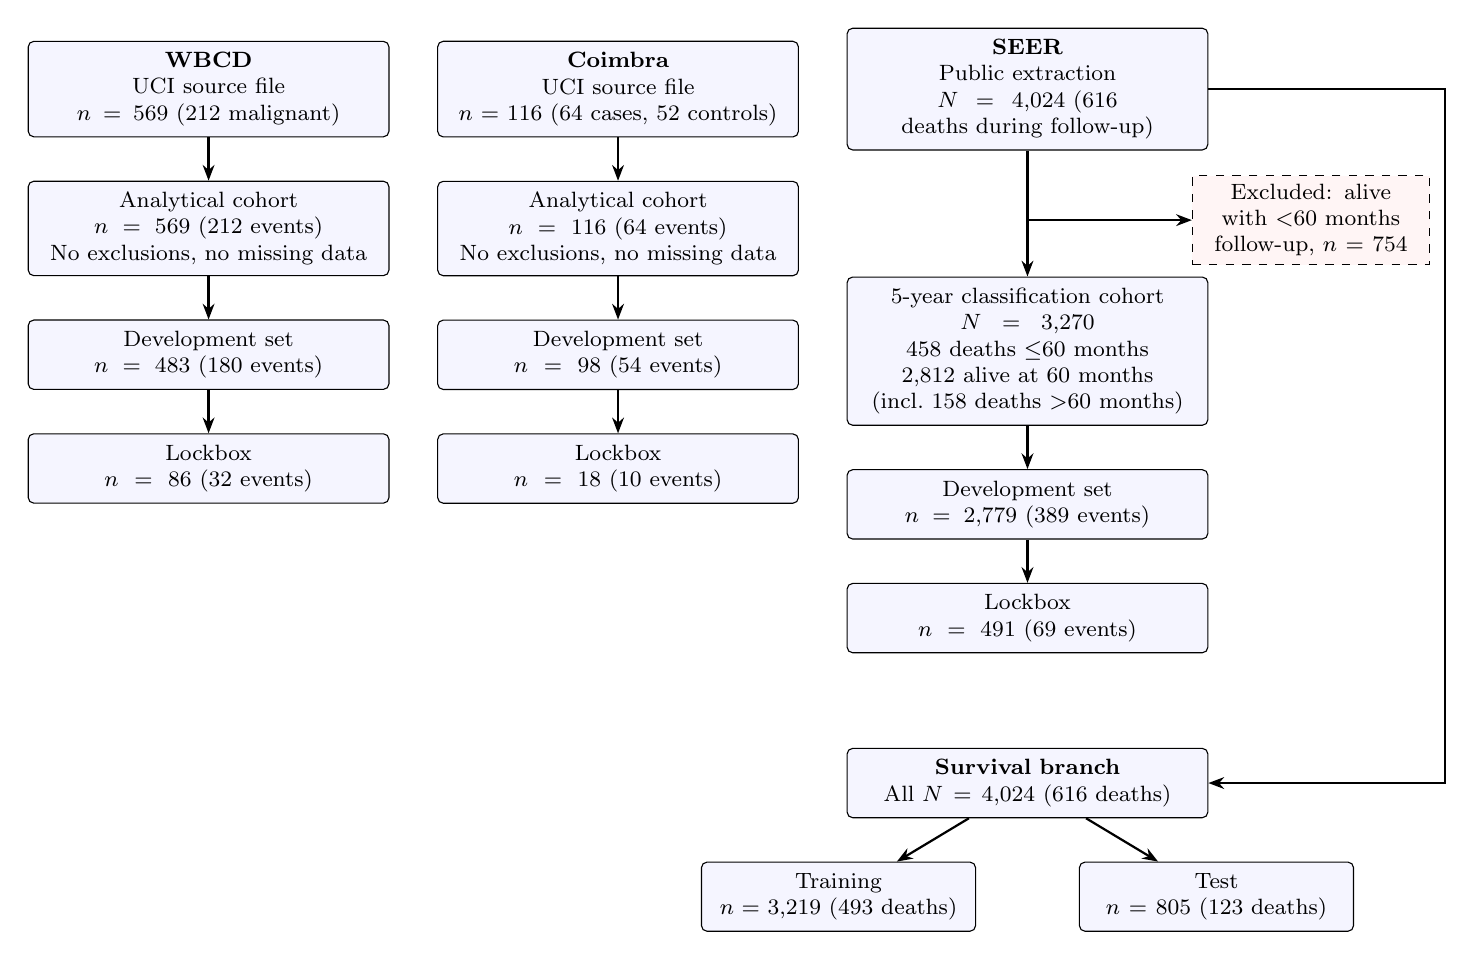
\begin{tikzpicture}[b/.style={draw,rounded corners=2pt,align=center,text width=4.3cm,font=\footnotesize,inner sep=4pt,fill=blue!4},
 e/.style={draw,dashed,align=center,text width=3.4cm,font=\footnotesize,inner sep=3pt,fill=red!4},
 a/.style={-{Stealth[length=2mm]},thick},node distance=0.55cm]
% WBCD
\node[b] (w1) at (0,0) {\textbf{WBCD}\\UCI source file\\$n=569$ (212 malignant)};
\node[b,below=of w1] (w2) {Analytical cohort\\$n=569$ (212 events)\\No exclusions, no missing data};
\node[b,below=of w2] (w3) {Development set\\$n=483$ (180 events)};
\node[b,below=of w3] (w4) {Lockbox\\$n=86$ (32 events)};
\draw[a] (w1)--(w2); \draw[a] (w2)--(w3); \draw[a] (w3)--(w4);
% Coimbra
\node[b] (c1) at (5.2,0) {\textbf{Coimbra}\\UCI source file\\$n=116$ (64 cases, 52 controls)};
\node[b,below=of c1] (c2) {Analytical cohort\\$n=116$ (64 events)\\No exclusions, no missing data};
\node[b,below=of c2] (c3) {Development set\\$n=98$ (54 events)};
\node[b,below=of c3] (c4) {Lockbox\\$n=18$ (10 events)};
\draw[a] (c1)--(c2); \draw[a] (c2)--(c3); \draw[a] (c3)--(c4);
% SEER
\node[b] (s1) at (10.4,0) {\textbf{SEER}\\Public extraction\\$N=4{,}024$ (616 deaths during follow-up)};
\node[b,below=1.6cm of s1] (s2) {5-year classification cohort\\$N=3{,}270$\\458 deaths $\le$60 months\\2,812 alive at 60 months\\(incl.\ 158 deaths $>$60 months)};
\node[e,text width=2.8cm] (ex) at ($(s1)!0.5!(s2)+(3.6,0)$) {Excluded: alive with $<$60 months follow-up, $n=754$};
\draw[a] (s1)--(s2); \draw[a] ($(s1)!0.5!(s2)$)--(ex.west);
\node[b,below=of s2] (s3) {Development set\\$n=2{,}779$ (389 events)};
\node[b,below=of s3] (s4) {Lockbox\\$n=491$ (69 events)};
\draw[a] (s2)--(s3); \draw[a] (s3)--(s4);
\node[b,below=1.2cm of s4] (v1) {\textbf{Survival branch}\\All $N=4{,}024$ (616 deaths)};
\node[b,below=of v1,xshift=-2.4cm,text width=3.2cm] (v2) {Training\\$n=3{,}219$ (493 deaths)};
\node[b,below=of v1,xshift=2.4cm,text width=3.2cm] (v3) {Test\\$n=805$ (123 deaths)};
\draw[a] (s1.east)--++(3.0,0)|-(v1.east);
\draw[a] (v1)--(v2); \draw[a] (v1)--(v3);
\end{tikzpicture}}
\end{center}
\captionof{figure}{Participant flow for the three cohorts and the SEER survival branch. Events are malignancy (WBCD), breast cancer (Coimbra), death from any cause within 60 months (SEER classification) and death from any cause during follow-up (survival branch).}

\newpage
\section*{Table S3. Participant characteristics by partition}
\addcontentsline{toc}{section}{Tables S3/S3b. Participant characteristics}
SMD: standardised mean difference between development and lockbox (continuous variables). Characteristics by case/control status for Coimbra are reported in the source publication (Patr\'icio et al., BMC Cancer 2018).
{\small
\begin{longtable}{@{}P{7.4cm}P{3.3cm}P{3.3cm}P{1.2cm}@{}}
\toprule
\textbf{Characteristic} & \textbf{Development} & \textbf{Lockbox} & \textbf{SMD}\\
\midrule\endhead
\bottomrule\endfoot
\inputrows{s3_rows.tex}
\end{longtable}
}

\subsection*{Table S3b. SEER classification cohort by race}
{\small
\begin{tabularx}{\textwidth}{@{}lllYYYY@{}}
\toprule
\textbf{Race} & \textbf{$n$} & \textbf{Age, mean} & \textbf{T3--T4 (\%)} & \textbf{N3 (\%)} & \textbf{ER negative (\%)} & \textbf{Death $\le$60 mo (\%)}\\
\midrule
\inputrows{s3b_rows.tex}
\bottomrule
\end{tabularx}
}

\section*{Table S4. Participants and events in each analysis}
\addcontentsline{toc}{section}{Table S4. Participants and events per analysis}
{\small
\begin{tabularx}{\textwidth}{@{}Ylll@{}}
\toprule
\textbf{Analysis set} & \textbf{WBCD} & \textbf{Coimbra} & \textbf{SEER 5-year}\\
\midrule
Analytical cohort & 569 (212) & 116 (64) & 3,270 (458)\\
Development set & 483 (180) & 98 (54) & 2,779 (389)\\
Outer CV training fold (approx.) & 386 (144) & 78 (43) & 2,223 (311)\\
Outer CV test fold (approx.) & 97 (36) & 20 (11) & 556 (78)\\
Inner tuning folds (approx., training / validation) & 257 / 129 & 52 / 26 & 1,482 / 741\\
Conformal: proper training / calibration / test & 289 / 97 (36) / 97 & 58 / 20 (11) / 20 & 1,667 / 556 (78) / 556\\
Lockbox model: training / conformal calibration & 386 (144) / 97 (36) & 78 (43) / 20 (11) & 2,223 (311) / 556 (78)\\
Lockbox & 86 (32) & 18 (10) & 491 (69)\\
SEER survival: training / test & -- & -- & 3,219 (493) / 805 (123)\\
\bottomrule
\end{tabularx}
}
Numbers are participants (events). Approximate values are for a typical fold of stratified splitting.

\newpage
\section*{Table S5. Cross-validated performance with Nadeau--Bengio corrected 95\% CIs}
\addcontentsline{toc}{section}{Table S5. Corrected confidence intervals}
The v1.0 manuscript reported percentile-bootstrap intervals over outer-fold scores, which treat correlated folds as independent and are too narrow. The intervals below use the corrected variance $S^2(1/n+1/(K-1))$ with $K=5$.
{\small
\begin{longtable}{@{}lllllll@{}}
\toprule
\textbf{Cohort} & \textbf{Label} & \textbf{Pipeline} & \textbf{Metric} & \textbf{Mean} & \textbf{SD} & \textbf{95\% CI (corrected)}\\
\midrule\endhead
\bottomrule\endfoot
\inputrows{s5_rows.tex}
\end{longtable}
}

\section*{Table S6. Conformal coverage by outcome class and subgroup (SEER, 100 iterations)}
\addcontentsline{toc}{section}{Table S6. Conformal coverage by subgroup}
{\small
\begin{tabularx}{\textwidth}{@{}llYYYY@{}}
\toprule
\textbf{Variable} & \textbf{Group} & \textbf{Coverage (\%)} & \textbf{Coverage in deaths (\%)} & \textbf{Coverage in survivors (\%)} & \textbf{Ambiguous sets (\%)}\\
\midrule
\inputrows{s6_rows.tex}
\bottomrule
\end{tabularx}
}
Coverage is marginal by construction; the large difference between deaths and survivors motivates class-conditional (Mondrian) conformal prediction in future work.

\section*{Table S7. Leakage and selector contrasts}
\addcontentsline{toc}{section}{Table S7. Leakage and selector contrasts}
{\small
\begin{tabularx}{\textwidth}{@{}lllYYll@{}}
\toprule
\textbf{Cohort} & \textbf{Label} & \textbf{Contrast} & \textbf{Mean difference} & \textbf{95\% CI} & \textbf{$p$ (two-sided)} & \textbf{$p_{\text{TOST}}$}\\
\midrule
\inputrows{s7_rows.tex}
\bottomrule
\end{tabularx}
}
Nested PCA $-$ Leaky isolates the effect of fitting scaling and PCA outside the folds (post hoc, descriptive). Unified $-$ Leaky combines leakage with adaptive selector choice. Margins: $\pm0.02$ accuracy, $\pm0.01$ AUROC. $p$-values unadjusted.

\newpage
\section*{S8. SEER label audit, v1.0 results and reproduction check}
\addcontentsline{toc}{section}{S8. SEER label audit and v1.0 results}
\textbf{Audit.} In the v1.0 code (\texttt{src/trust\_bc\_multicohort\_benchmark.py}), the SEER label was \texttt{y = (Status == 'dead')} after excluding patients alive with fewer than 60 months of follow-up. Of the 616 deaths, 458 occurred at or before month 60 and 158 occurred between months 61 and \seerMaxDeathMonth. These 158 patients were alive at the 5-year horizon but were labelled as 5-year deaths, so the v1.0 endpoint was ``death at any time during follow-up among patients with at least 60 months of follow-up or an observed death'' rather than 5-year mortality.

\textbf{Correction.} Version 1.1 labels an event only if death occurred at or before month 60. The analytical cohort size is unchanged ($N=3{,}270$) but the number of events falls from 616 to 458 and the prevalence from 18.8\% to 14.0\%.

\textbf{Reproduction check.} The v1.1 re-analysis re-implemented the Leaky, Nested PCA, Nested RF and Unified pipelines with identical code, seeds and splits (\texttt{scripts/seer\_revision\_core.py}) in a newer software environment (scikit-learn 1.8.0). Run with the v1.0 label, it \seerReproText{} The split manifest was also reproduced exactly (491 identical lockbox indices).

\subsection*{Table S8. SEER results under the v1.0 label (as originally reported)}
{\small
\begin{tabularx}{\textwidth}{@{}lYYYYY@{}}
\toprule
\textbf{Pipeline} & \textbf{AUROC mean $\pm$ SD} & \textbf{95\% CI (corrected)} & \textbf{Holm $p$ vs Leaky} & \textbf{Holm $p$ vs Unified} & \textbf{Brier / ECE}\\
\midrule
Leaky baseline & 0.718 $\pm$ 0.024 & 0.692--0.744 & -- & -- & 0.155 / 0.133\\
Tuned XGBoost & 0.732 $\pm$ 0.027 & 0.703--0.761 & 0.5011 & 1.0000 & 0.140 / 0.022\\
Tuned LightGBM & 0.731 $\pm$ 0.027 & 0.702--0.760 & 0.5011 & 1.0000 & 0.149 / 0.052\\
Nested PCA-only & 0.718 $\pm$ 0.025 & 0.691--0.744 & -- & -- & 0.155 / 0.133\\
Nested RF-only & 0.732 $\pm$ 0.023 & 0.707--0.757 & -- & -- & 0.152 / 0.128\\
Unified & 0.732 $\pm$ 0.023 & 0.707--0.757 & 0.2939 & -- & 0.152 / 0.128\\
\bottomrule
\end{tabularx}
}
v1.0 TOST (Unified vs Leaky): $p=0.7116$. v1.0 lockbox: accuracy 80.04\%, AUROC 0.731, sensitivity 34.78\% (32/92), specificity 90.48\% (361/399), conformal coverage 96.54\%; v1.0 conformal (development): coverage 95.32\%, singleton 48.62\%, ambiguous 51.38\%.

\textbf{Effect of the correction.} Discrimination was similar (Unified AUROC 0.732 $\rightarrow$ \seerUniAUC), but the proportion of ambiguous conformal sets fell from 51.38\% to \seerConfAmb\%, and the Unified selector chose RF in \seerRFfolds/35 rather than 35/35 folds. The v1.0 claim of a leakage effect in SEER (Unified vs Leaky, 0.732 vs 0.718) is explained by the selector: under both labels the architecture-matched contrast was essentially zero (Table S7).

\begin{center}
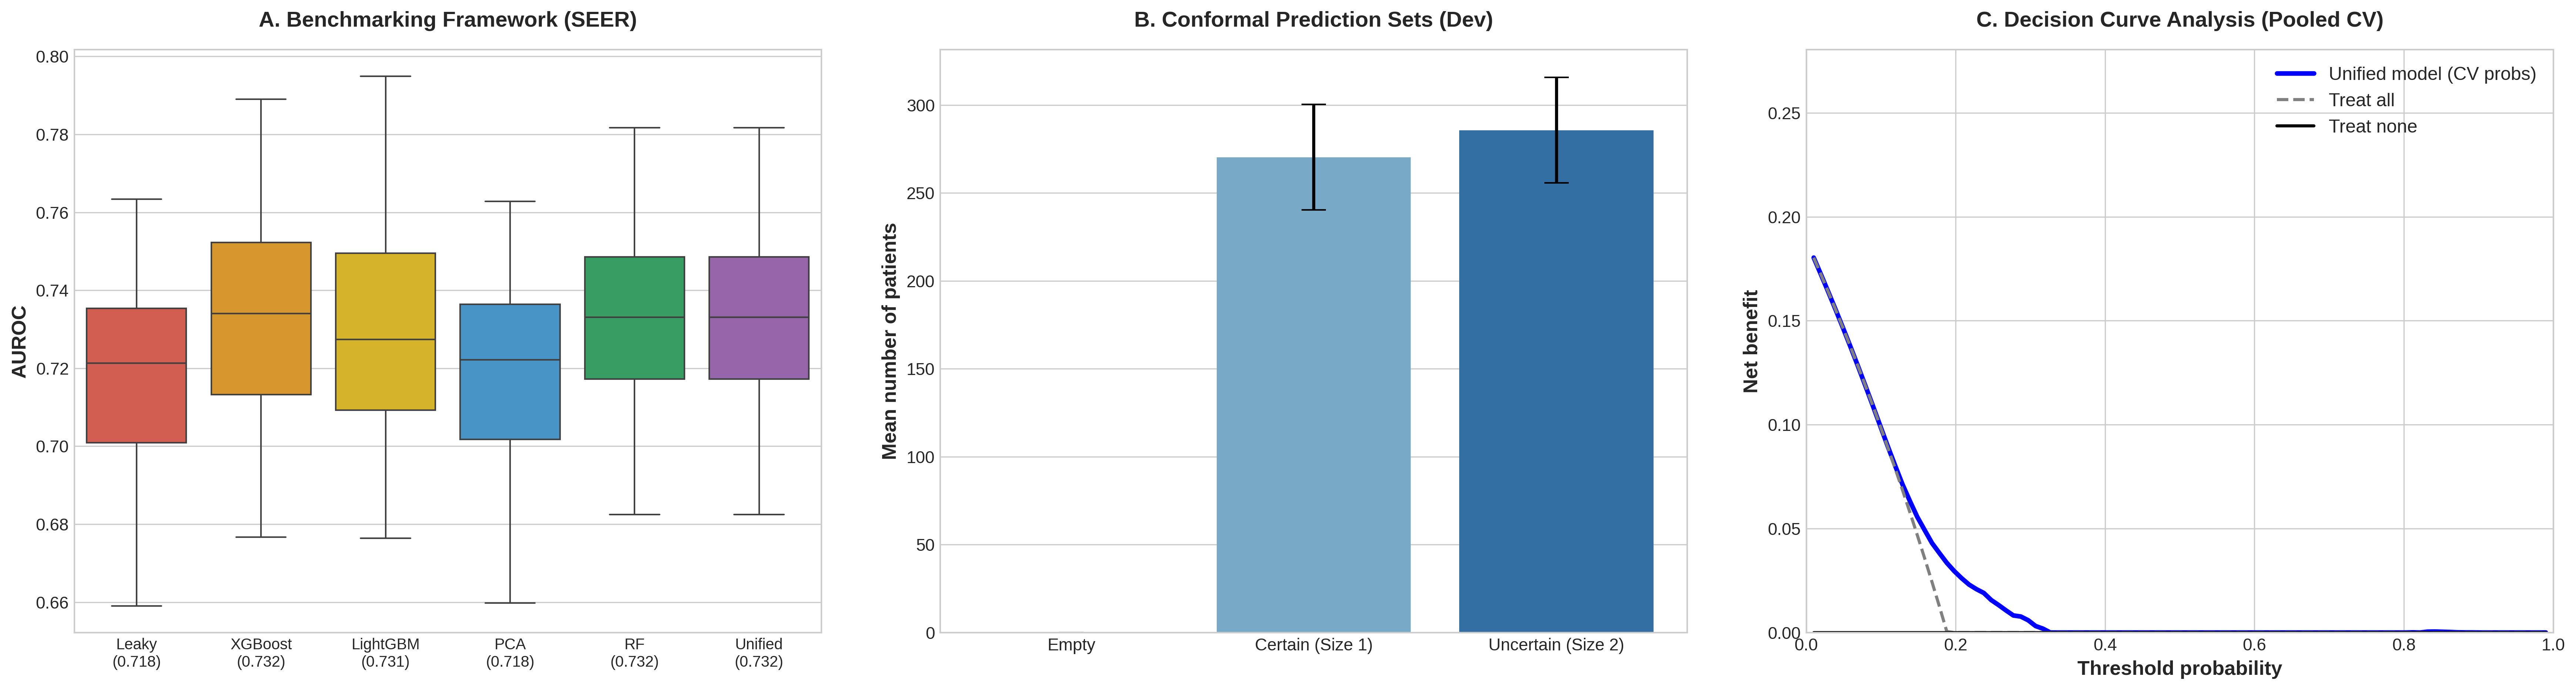
\includegraphics[width=0.95\textwidth]{figs/SEER_fig_main_v1.png}
\captionof{figure}{SEER results under the v1.0 label (original Figure 2c), retained for transparency.}
\end{center}

\section*{Table S9. Minimum sample size for model development (Riley et al.)}
\addcontentsline{toc}{section}{Table S9. Minimum sample size}
Cox--Snell $R^2$ derived from the anticipated C statistic by simulation (Riley, Van Calster \& Collins, Stat Med 2021). Criteria: (i) shrinkage $\ge0.90$; (ii) optimism in Nagelkerke $R^2\le0.05$; (iii) overall risk within $\pm0.05$.
{\small
\begin{tabularx}{\textwidth}{@{}lYYYYYYY@{}}
\toprule
\textbf{Cohort} & \textbf{Parameters} & \textbf{C} & \textbf{Prevalence} & \textbf{$R^2_{CS}$} & \textbf{$n$ (i) / (ii) / (iii)} & \textbf{Required} & \textbf{Available (dev)}\\
\midrule
WBCD & 30 & 0.99 & 0.373 & 0.659 & 228 / 479 / 360 & 479 & 483\\
Coimbra & 9 & 0.79 & 0.552 & 0.244 & 286 / 206 / 381 & 381 & 98\\
SEER 5-year & 16 & 0.73 & 0.140 & 0.083 & 1,645 / 544 / 186 & 1,645 & 2,779\\
\bottomrule
\end{tabularx}
}
For evaluation, at least 100 events and 100 non-events are commonly recommended; the lockboxes contain 32, 10 and 69 events.

\end{document}
